%% 和文論文用のテンプレート
%%%%%%%%%%%%%%%%%%%%%%%%%%%%%%%%%%%%%%%%%%%%%%%%%%%%%%%%%%%%%%%%%%%%%%%%%%%%
%% 1. 和文原稿
 \documentclass[originalpaper]{jsaiart}     % 原著論文 Original Paper
% \documentclass[blindreview]{jsaiart}      % 査読用
%
% \documentclass[shortpaper]{jsaiart}       % 速報論文 Short Paper
% \documentclass[exploratorypaper]{jsaiart} % 萌芽論文 Exploratory Research Paper
% \documentclass[Specialissue]{jsaiart}     % 特集 Special Issue
% \documentclass[specialissue]{jsaiart}     % 小特集 Special Issue
% \documentclass[interimreport]{jsaiart}    % 報告 An Interim Report
% \documentclass[surveypaper]{jsaiart}      % 解説 Survey Paper
% \documentclass[aimap]{jsaiart}            % AIマップ AI map
% \documentclass[specialpaper]{jsaiart}     % 特集論文 Special Paper
% \documentclass[invitedpaper]{jsaiart}     % 招待論文 Invited Paper
%

%% ページ番号の指定,掲載時に学会の方で決定します.
% \setcounter{page}{1}
% \setcounter{volpage}{1}


%%% amsmathパッケージの注意点 %%%%%%%%%%%%%%%%%%%%%%%%%%%%%%%%%%%%%%%
% \usepackpage{amsmath}
% 数式番号の参照は \ref ではなく,\eqref を用いること
% documentclass のオプションに fleqnを指定すること
% 例: \documentclass[technicalpaper,fleqn]{jsaiart}

\usepackage[dvipdfmx]{graphicx}
\usepackage{graphics}
\usepackage{fancybox}
\usepackage{comment}

\Vol{12}
\No{1}
%\jtitle{物体検出のためのニューラルネットワークのサーベイ}
\jtitle{物体検出に用いられるニューラルネットワークモデル}
% \jtitle[柱用和文タイトル]{和文タイトル}
\jsubtitle{最新モデルのサーベイと目的に応じたモデルの選択}
%\etitle{A Survey of Deep Neural Networks for Object Detection}
\etitle{Neural Network Models for Object Detection}
\esubtitle{A Survey of the Latest Models and Optimal Model Selections for Specific Tasks}

\manyauthor % 著者が3名以下の場合はこの行を消すこと

%%% 著者名の注意点 %%%%%%%%%%%%%%%%%%%%%%%%%%%%%%%%%%%%%%%%%%%%%%%%%%%
% 所属先が同じ著者が連続する場合,その中の先頭の著者のみ \affiliation
% を用い,残りの所属先には \sameaffiliation を使う
% ただし,所属先が同じでも連続していない場合は \affliation を使う
% 名前が長い場合は \name の代りに \longname を使う

\author{%
 \name{金子}{純也}{Junya Kaneko}
 \affiliation{Morning Project Samurai 株式会社}%
     {Morning Project Samurai Inc.}%
     {junya@mpsamurai.com, http://www.mpsamurai.com}
%\and
% \name{著者2姓}{名}{Auther2 Roman Name}
% \affiliation{日本語所属名2}%
%     {Affiliation2 in English}%
%     {user2@ai-gakkai.or.jp, http://www.ai-gakkai.or.jp/~user2/}
\and
 \name{山田}{貢己}{Miki Yamada}
 \sameaffiliation{m.yamada@mpsamurai.com}
%\and
% \longname{カタガナガキノ}{ナガイナガイナマエ}{VeryLong Roman Name}
% \sameaffiliation{user4@ai-gakkai.or.jp, http://www.ai-gakkai.or.jp/~user4/}
%\and
% \name{著者5姓}{名}{Auther5 Roman Name}
% \affiliation{日本語所属名1}%
%     {Affiliation1 in English}%
%     {user5@ai-gakkai.or.jp, http://www.ai-gakkai.or.jp/~user5/}
}

\begin{keyword}
%キーワードとして,小文字(固有名詞や略語を除く)の英単語を2〜5個指定
    survey, neural network, object detection, instance segmentation, deep learning
\end{keyword}

\begin{summary}
「ショートノート」は 200 ワード,それ以外は200〜500 ワード
以内の英文でsummaryを記す
(ここは,論文執筆後に書く.)
\end{summary}

\begin{document}
\maketitle

★ここにチートシートを出力する.
\section{まえがき}
%■ 本論文の目的:誰(理工系大学2年生)を対象に、何(物体検出の始め方)を伝えるか
%\subsubsection*{この論文の狙い}
{\bf この論文の狙い:\ }このサーベイは,理工系大学2年生程度の数学の知識を前提に,物体検出をこれから始めるにはどうすればよいかという道すじを伝えることを目的として執筆したものである.物体検出でできることは何?から始まり,物体検出をするために必要なもの(ハード,ソフト,データ,知識,明確な目的)を簡潔に纏めてある.また,読者にとっての理想的なサーベイ(即時性,分かりやすさ,一言で説明,参考文献は充実)というものの一つの解として,随時更新されるGitHub上の(日本語で書かれた)物体検出まとめサイトとライブラリを紹介する.

%■ 最近の世の中の状況のおさらい
{\bf 世の中の状況:\ }近年,「AI(人工知能)」という言葉が国内外に蔓延しており,技術者のみならず一般の人の日常生活にもすっかり浸透した.常に手の届くところにAIがあり,AIに囲まれて生活していると言っても過言ではない.テレビやインターネットの画像は,本物と見間違えるほどの人工画像で溢れ,スマホや机上のスピーカーに話しかけるとあらゆる情報を教えてくれるばかりでなく,電化製品を操作することもできるようになった.高速道路を自動運転する車も増えている.

%■ AI分野(画像認識分野)における物体検出の位置づけ
{\bf AI分野における物体検出:\ }ここ数年で飛躍的に性能を向上させたAI関連技術は,画像認識,物体検出,ロボット制御,音声認識,機械翻訳,ビッグデータ分析などであり,これらの多くの領域で深層ニューラルネットワーク(Deep Neural Network(DNN))が使われている.とりわけ画像認識分野でこのDNNが注目されるようになったのは,2012年に開催された最先端の一般物体認識の性能を競うコンテスト ILSVRC においてDNNを使った手法が他の手法に大差をつけて優勝したことが発端である.「画像中の物は何か?」に答える物体認識をさらに進めて,「画像中のどこに何があるか?」に答えようとするものが本論文のテーマ「物体検出」であり,現在のAIブームを巻き起こした源流がここにあると言ってよい.

%■ 物体検出でできること
{\bf 物体検出でできること:\ }物体検出とは,カメラで撮影された画像データを電子的に処理し,予め登録しておいた物体(例えば,人,犬,猫,自動車,飛行機,...)を見つけ出し,その正確な画像上の位置と物体の種類を予測するものである(「予測(predict)」は,「推定(estimate)」,「推論(inference)」などとも呼ばれ全て同じ意味で使われる).

現在の標準的方法においては,予め,検出したい対象の学習データ(物体が写っている画像,物体の種類,物体の位置を示す矩形の座標)を大量に用意し,画像を入力すれば種類と位置を出力するように,ニューラルネットワーク等の予測モデルを学習させる.通常,これに数時間から数日要すると言われている.

学習が完了した予測モデルの能力は,タスクの種類によっては人間の能力(予測結果のスコアの平均値)を超えたと言われているものもある(物体認識など).ただし,物体が写し出された画像の品質(解像度,ノイズ,露出不足/過多)や撮影アングル(遮蔽物,変形,大き(小さ)過ぎる)に問題がある場合は性能が低下することは避けられない.

物体検出と似た技術として,次の3つがある:

\begin{itemize}
    \item セマンティックセグメンテーション(全画素の物体の種類を認識するが,同種の物体同士は区別しない)
    \item インスタンスセグメンテーション(同種の異なる個体を区別して物体検出を行い,且つ,画素単位で個体の識別をする)
    \item パノプティックセグメンテーション(全画素の物体の種類を認識し,同種の異なる個体も区別する)
\end{itemize}
本論文では上記のセグメンテーション技術も含めた広い意味での物体検出について述べる.

%■ 物体検出をするために必要なもの(ハード、ソフト、データ、知識、明確な目的)
{\bf 物体検出をするために必要なもの:}

\begin{description}
    \item[ソフトウェア] 
    \begin{itemize}
        \item PyTorch/TensorFlow 等の深層学習ライブラリとその稼働環境(Linux/Windows/Mac上のPython, jupyter notebook環境など).
        \item 物体検出を行うソフトウェア(予測モデルの作者,または,物体検出を行おうとする担当者が作ったもの).
    \end{itemize}
    \item[ハードウェア] 
    \begin{itemize}
        \item 前記ソフトウェアが実行できる環境(PC(GPUがあると良い), 或いは,Google Corabolatory などのサーバ上の実行環境).
    \end{itemize}
    \item[データ] 
    \begin{itemize}
        \item 学習データ(事前学習用,並びに,fine-tuning用の入力と出力のペア)
        \item 本来処理したいデータ(入力).
    \end{itemize}
    これらは,使用するソフトウェアで読み取ることのできる状態にしておく(データの前処理).
    \item[知識] 物体検出のソフトウェアを使うには,入出力データの意味を理解する必要がある.特に,予測モデルの出力データは通常は誤差を含むものとなるため,出力が表す数値が確率値を表すのか,何らかの物理量を表すのか,分類のカテゴリを表すのか,正確に把握する必要がある.また,学習時の損失関数の値から,予測モデルの推定誤差を見積もることができるのだが,それには出力結果を正しく解釈できる統計学の知識が必要となる.
    \item[明確な目的] 何がしたいのかということを明確化しておくことがが,物体検出を行おうとするときに重要となる.物体検出は新しい技術であり,標準的な統計解析の手法よりも手間と計算コストが大きくなりがちである.他の方法では解決できないのか?と問いかけて,本当にこれが必要であることを確認しておくべきである.
\end{description}

%■ 良いサーベイとは(即時性、分かりやすさ、一言で説明+参考文献)(随時更新する)まとめサイトとライブラリ(GitHub)の紹介。
{\bf 理想的なサーベイとは:\ }最新技術のサーベイ論文は,有用であり様々な分野で昔から(論文雑誌が生まれた頃から)活用されていると思われる.しかしながら,進歩の速い分野においてはサーベイが出た頃には既に内容が古くなってしまっているという問題が往々にして起こる.また,とても良く書かれたサーベイほど内容が濃く多くなり,執筆に時間と労力を要するのはもちろん,それを読み解くのにも時間を要するということもよくある.

我々は,github上に随時更新される形式でサーベイを公開することを試みた.出版されたときには既に古くなっているという懸念を取り払える可能性を期待している.また,この分野に新規参入しようとしている人がなるべく短時間で必要な情報にたどり着き,取り組んでいる問題を解決する最適な方法を見つけたり,或いは,新たな研究に取り組めることを目指し,内容の拡充性や緻密性よりも,なるべく視覚的に解りやすいコンパクトな内容になるよう心掛けた.

\section{物体検出(Object detection)}
%\begin{figure}[t]
%    \begin{center}
%        \includegraphics[width=8cm,clip]{fig/test_fig2.eps}
%    \end{center}
%    \caption{ 図の説明文 ... }
%\end{figure}
\subsection{物体検出器(object detector)の働き}
{\bf 基本動作:\ }物体検出器は,画像(1枚の静止画をファイルにしたもの)を処理し,処理結果(検出個数,検出物体の画像座標,検出物体の種類)を出力する.セグメンテーションの場合は,出力解像度(画像のサイズ)に応じた各画素のクラス分類結果も出力される.画像を読み込ませる際には,幅と高さを含む情報も与える必要がある.検出器によっては画像サイズや画像ファイル形式が指定されているものもあるのでその場合は,予め画像ファイルを変換する前処理が必要となる.

{\bf 出力結果の見かた:\ }検出座標は物体を囲む矩形(bounding box)の座標を4つの数値で表すことが多い.また,検出の信頼度が[0,1]の実数で出力される場合はそれが推定正答確率を表すように設定されている.

{\bf 学習のしかた:\ }学習データは,推論実行に必要なデータに正解データを加えたものであり,いわゆる教師あり学習を行わせる.ただ,推論時には無い学習に関するパラメタの設定をしなければならない.検出器の構成(中間層の層数,特徴量次元のサイズ,検出器独自のパラメタなど)もこの段階で設定する.通常は,確率的降下法でモデルのパラメタを学習させることが多く,検出器の重みパラメタの初期化方法(平均,分散,値を指定など),最適化方法(SGD, Adam, 他),学習率のスケジューリング,学習打ち切り基準,ミニバッチサイズなどを指定する.学習時には交差検証を行わせて未学習データに対する誤差も計算させることができるので,その誤差を控えておくことにより推論時の予測精度を見積もることができる.

{\bf 事前学習(pre-training)と事後学習(post-training, fine-tuning):\ }世界最高性能を出すほどの検出器の学習は,たいてい事前学習と事後学習の2段階で行われる.事前学習は主に公開データベースなどの大量データを用いて検出器の前半部分を学習させて適切な内部表現を獲得するために行われる.検出器によっては事前学習済みの重み係数パラメタが公開されているものもある.事後学習は,最終目的に合致したデータを追加して,場合によっては検出器の最終層を追加して,所望の検出処理を実行できるように最終調整の意味合いで実施するものである.事前/事後学習のやり方は各検出器によって異なるため,説明書きや論文等に記された方法を参考にして実行する必要がある.
\subsection{Two-stage検出器}
\subsubsection{Faster R-CNN}
\subsubsection{TFANet}
\subsubsection{Few-Shot Object Detection}
\subsection{One-stage検出器}
\subsubsection{YOLOv4}
\subsubsection{EfficientDet}
\section{インスタンスセグメンテーション(Instance segmentation)}
\subsection{Mask Scoring R-CNN (MS R-CNN)}
%\begin{figure*}[b] %これにすると独立したページに1段組で出力された.
\begin{figure}[b]
    \begin{center}
        \includegraphics[width=8cm,clip]{fig/archi_ms_rcnn.eps}
    \end{center}
    %\capwidth=90mm %
    \caption{ Mask Scoring R-CNN の構造.}
    %\end{figure*}
    \label{fig:archi_ms_rcnn}
\end{figure}
マスク品質(インスタンスマスクと正解マスクとのIoUとして定量化されるもの)を分類スコアと明示的に関連付けたモデルである\cite{HHGHW19}.MS R-CNN は,予測マスクの品質を学習するためのブロック(MaskIoU Head)を,Mask R-CNN\cite{HGDG17} に導入したモデルになっている(\ref{fig:archi_ms_rcnn}).MaskIoU Headはインスタンスの特徴量と対応する予測マスクを一緒に取り込み,それを元にMask IoU を回帰推定する.そして,推論時に予測MaskIoUを分類スコアに掛け算して補正する.
\subsubsection{MS R-CNN の学習}
学習サンプルとして RPN proposals を使う.
proposal box と正解box との IoU が 0.5 以上の学習サンプルが必要となる.これは Mask R-CNN の Mask head の学習サンプルの場合と同じである.
各学習サンプルに対する回帰目標を生成するために,まず目標クラスの予測マスクを取得し,予測マスクを閾値=0.5で2値化する.そして,2値化マスクと正解との MaskIoU を使う.
MaskIoUを回帰するのには L2 損失を使い,損失重みは1にする.
ネットワーク全体は end-to-end で学習する.
\subsubsection{MS R-CNN の推論処理}
MaskIoU Head は分類スコア(R-CNN head の出力)の調整に使う.推論の手順は次のようになる:
\begin{enumerate}
    \item R-CNN head が $N$個のbounding boxを出力する.
    \item $N$個のbounding boxのうち,SoftNMS\cite{BSCD17}で上位$k$個のボックスを選択する.
    \item 上位$k$個のボックスを Mask Head に入力し,$k$個のマルチクラスマスクを生成する(ここまでは標準的 Mask R-CNN の手順).
    \item これら$k$個のマスクを目標として MaskIoU Head に入力し,予測 MaskIoU を出力する.
    \item 予測 MaskIoU を,分類スコアに掛け算し,上位$k$個の修正された分類スコアを得る.
\end{enumerate}

\subsection{YOLACT++}
\section{パノプティックセグメンテーション(Panoptic(?) segmentation)}
\section{むすび}

\begin{acknowledgment}
謝辞について
\end{acknowledgment}

%\bibliography{btxsample}
\bibliography{mps}
\bibliographystyle{jsai}

\appendix

\section{付録のタイトル1}
付録の本文1
%\section{付録のタイトル2}
%付録の本文2

% 著者の姓と名の間は半角スペースで区切る
% 略歴は200字以内
\begin{biography}
    %\profile*{m}{著者姓 名}{前掲\kern-.5zw (Vol.X,No.Y,p.Z)\kern-.5zw 参照.}
\profile{m}{金子 純也}{著者1の略歴}
\profile{m}{山田 貢己}{1989年東京大学大学院物理学専攻修了.理学博士.同年株式会社東芝入社.ニューラルネットワークの研究開発,セキュリティ技術,画像認識技術,テレビの高画質化技術,車載画像認識プロセッサ等の開発業務に従事.2020年ジャパニアス株式会社に入社.現在,Morning Project Samurai 株式会社においてAI開発業務に従事.}
\end{biography}

\end{document}
